%!TEX root = ../Thesis.tex
\section{Dokumentation der Software}

\subsection{Dokumentation der Paketstruktur des Android-Projektes [Falk]}

Die Applikation liegt im Paket \code{de.fhdw.wip.rpntilecalculator} und ist in einzelne Klassen unterteilt, welche in eine Ordnerstruktur eingebettet sind. Diese Ordnerstruktur orientiert sich an dem gewählten UI Design Pattern MVP. Dabei gibt es einen Model Ordner. Dieser ist in vier weitere Ordner unterteilt, welche den Kachelarten nachempfunden sind und einen für den Stack. In diesen befinden sich verschiedene Klassen, die zusammen das Model bilden. Im \code{Presenter}-Ordner befindet sich lediglich der Presenter. Der \code{View}-Ordner besteht wieder aus mehreren Teilen. Zum einen aus der \code{MainActivity}, welches die Hauptansicht der Appliaktion darstellt. Dazu befinden sich dort Typen und Grundklassen der Kacheln. Es gibt noch die drei Ordner \code{Layout}, \code{Menu} und \code{Schemes}. In \code{Layout} befinden sich Funktionen zum Darstellen, Speichern und Laden der Kacheln. In \code{Schemes} befinden sich Vorlagen für Tiles und in \code{Menu} sind sämtliche Menüs gespeichert. 

\begin{figure}[!h]
	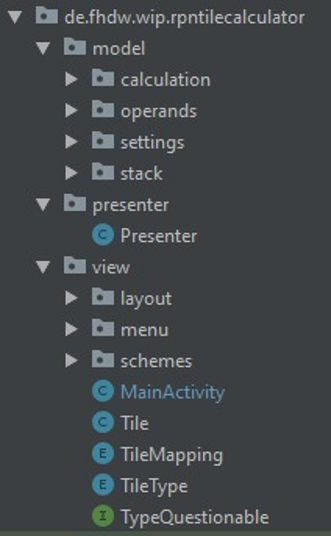
\includegraphics[scale=1]{img/ordnerstruktur}
	\caption[Ordnerstruktur]{Ordnerstruktur\footnotemark}
\end{figure}
\footnotetext{eigene Darstellung (Screenshot aus Android Studio)}

\begin{figure}[!h]
	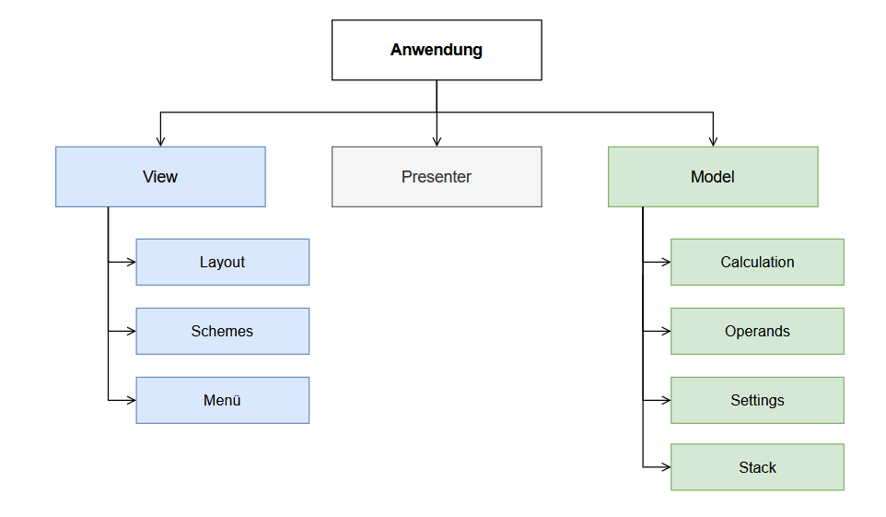
\includegraphics[scale=1]{img/ordnerstruktur2}
	\caption[Ordnerstruktur Schema]{Ordnerstruktur Schema\footnotemark}
\end{figure}
\footnotetext{eigene Darstellung}

\subsection{Dokumentation der View}

In den folgenden Kapiteln wird die Implementierung des Frontends der Applikation, der sogenannten View, und jeglichen zugehörigen Implementierungen, dargestellt.

\subsubsection{Activities [Bockhorn]}

Die Applikation wird durch den Aufruf der sogenannten \code{MainActivity} vom Android System beim Öffnen der Anwendung gestartet. Da die Menüführung nicht auf Activities basiert und jegliche Layouts dynamisch geladen werden, bleibt die \code{MainActivity} die einzige Activity der Applikation

Im MVP Pattern ist die \code{Activity} der View zugeordnet. Sie lädt unter anderem vertikale und horizontale Layouts vor und stellt eine Methode zur Darstellung dieser bereit. Auch wird ein Listener erstellt, der nach Änderungen der Bildschirmausrichtung horcht und passende Layouts lädt.

\paragraph{Klasse: MainActivity}

\textbf{Beschreibung:} Activity, die beim Starten der Anwendung aufgerufen wird und das Layout \code{activity\_main.xml} aufruft. Dieses Layout ist jedoch leer, da alle Inhalte dynamisch geladen werden. Es lädt auch Taschenrechner-Layouts vor und stellt Methoden zur Darstellung dieser bereit.

\textbf{Methode} \code{onCreate} lädt die Layouts vor, erstellt einen \code{Listener} ob die Orientierung sich verändert und öffnet das erste Layout.

\textbf{Methode} \code{setTileLayout} lädt ein Layout in die View.

\subsubsection{Generische Kachelgestaltung [Tom]}

Die generische Gestaltung der Kacheln wurde gemäß dem Entwurf so umgesetzt, dass eine Trennung zwischen Kacheln, die als Buttons vom Kontext der Applikation abhängig sind, und Kacheln, die vom Kontext unabhängig sind, ermöglicht wird. Dies dient unter anderem dem Vorladen von Layouts zur Optimierung der Ladeperformance. Außerdem wird so die Definition des Kacheltypen und dessen spezialisierte Inhalte auf die vom Kontext unabhängigen Kachelschemata (\code{TileSchemes}) ausgelagert. 

Als logische Abtrennung kann man sich merken, dass Kacheln (\code{Tiles}) lediglich für die Kommunikation mit dem Nutzer zuständig sind, während die \code{TileSchemes} die restliche Frontend-Logik beinhalten.

\subsubsection{Kontextbezogene Kacheln [Bockhorn]}

Die Tiles werden mit Bezug auf den Kontext, also die aktuell dargestellte Activity, erstellt. Sie dienen als generische Kachelklasse, dessen Funktionalitäten unabhängig vom Kacheltypen gebraucht werden.

Ein Tile, als Unterklasse des \code{AppCompatButton} von Android, wirft beim Anklicken ein Event, welches von registrierten \code{OnClickListenern} abgefangen werden kann. Für die einzelnen Tiles wird der \code{Presenter} als \code{OnClickListener} registriert, sodass dieser die vom Nutzer getätigten Klicke verarbeiten kann. Zusätzlich wird dem \code{Tile} als \code{OnLongClickListener} das Menü \code{TileTypeInput} übergeben, welches bei langem Klicken geöffnet wird und somit die Bearbeitung des Kacheltypen ermöglicht.

\begin{figure}[!h]
	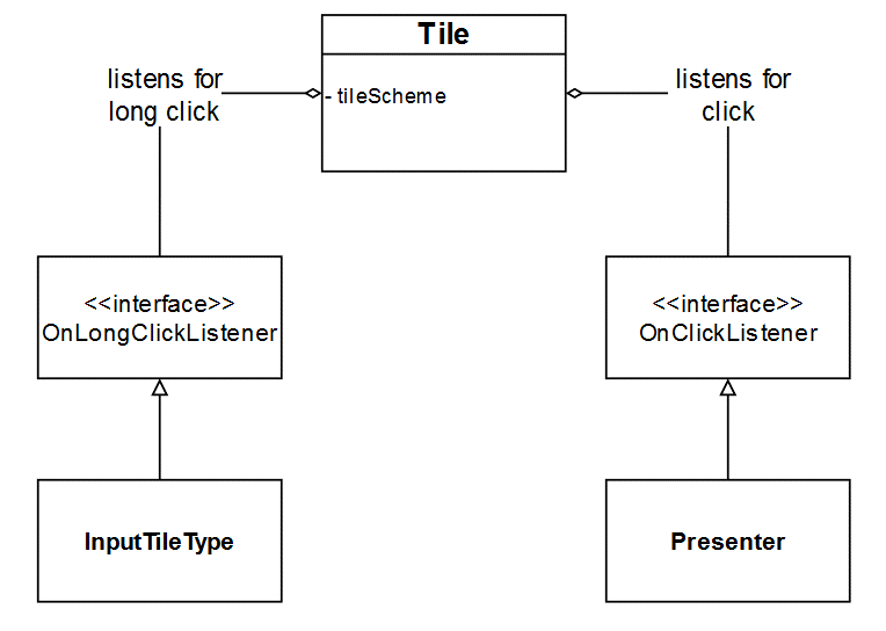
\includegraphics[scale=1]{img/listener-von-tile}
	\caption[Listener von Tile]{Listener von Tile\footnotemark}
\end{figure}
\footnotetext{eigene Darstellung}

Die Informationen über den Kacheltypen des \code{Tiles} befindet sich im \code{TileScheme} des \code{Tiles}. Werden nun die Inhalte, oder gar der Kacheltyp des \code{Tiles} verändert, so wird das Aussehen des \code{Tiles} anhand des aktuellen \code{TileSchemes} aktualisiert. Ähnlich stellt ein \code{Tile} verschiedene Animationen bereit, die zum Beispiel beim Laden oder Speichern des \code{Tiles} aufgerufen und abgespielt werden können.

\paragraph{Tile [Bockhorn]}

\textbf{Superklasse:} \code{AppCompatButton}

\textbf{Beschreibung:} Agiert als Button auf einem Kontext, dessen Inhalt und Typ durch ein \code{TileScheme} definiert sind. Einfaches Klicken wird vom \code{Presenter} abgefangen und gedrückt halten öffnet ein Auswahlmenü für die Kachelart. 

\textbf{Methode} \code{update} Aktualisiert das \code{Tile} mithilfe eines neuen \code{Schemes}. Setzt dabei Hintergrund Ressource und Text

\textbf{Methode} \code{enableMenulistener} Aktiviert die Menüfunktion für dieses \code{Tile}

\subsubsection{Kontextfremde Kacheln [Gentges]}

Die \code{TileSchemes} stehen in keiner Beziehung zum Kontext der Anwendung. Dennoch wird in ihnen der Text und das Design des letztendlichen \code{Tiles} gespeichert. Im Gegensatz zu den \code{Tiles} differenzieren \code{TileSchemes} hier zwischen Kachelarten. Die Grundeigenschaften eines \code{TileSchemes}, also die Information darüber um welche Art von Kachel es sich handelt, und was genau der Inhalt ist, werden in der Superklasse \code{TileScheme} definiert. Ersteres liegt in Form eines sogenannten \code{TileMappings} vor, welches in einem folgenden Kapitel näher erläutert wird XXX. Für jede der bestehenden Kachelarten wurde eine Unterklasse implementiert, welche die Eigenschaften von \code{TileScheme} erbt und weitere artbezogene Inhalte definiert. In Kombination mit einem \code{Tile} können so andere Komponenten der Applikation, wie beispielsweise der \code{Presenter}, die Kachelart des \code{TileScheme} erfragen und den vorliegenden Inhalt für die auszuführenden Prozesse extrahieren.

\begin{itemize}
	\item Das \code{ActionTileScheme} ist die Implementierung eines \code{TileScheme} vom Typ Action, (auch \code{Operator}) der Inhalt und Typ um eine instanziierte Action erweitert. Dank der ähnlich polymorphen Struktur der \code{Action}s, kann so mit einem simplen Methodenaufruf jede Form von \code{Action}, die im Schema hinterlegt ist, angesprochen und ausgeführt werden.
	\item Ein \code{SettingTileScheme} erbt ebenfalls von \code{TileScheme}, aber liefert zusätzlich Informationen über ein sogenanntes \code{Setting}, welches ähnlich wie eine \code{Action} über eine vererbte Methode anzusprechen ist.
	\item Ein \code{OperandTileScheme} ist gleich aufgebaut, beinhaltet aber Operanden, die als Grundlage für die Kalkulation mit \code{Action}s dienen.
	\item Das Klicken auf ein \code{Tile} des Stacks wird intern gleich gehandhabt, wie das Klicken eines Operanden. Jedoch besitzen Tiles aus dem Stack eine Reihenfolge, die im \code{StackTileScheme} als Rang hinterlegt wird. Um die gleiche Behandlung eines potenziellen Operanden im Stack zu gewährleisten, erbt \code{StackTileScheme} nicht von \code{TileScheme}, sondern von \code{OperandTileScheme}. 
	\item Ein \code{HistoryStackTile} ist ebenfalls so aufgebaut, wie ein \code{StackTileScheme}, und erbt daher dessen \code{Attribute}.
\end{itemize}

Die Erstellung einzelner \code{TileSchemes} erfolgt mithilfe des Factory Method Design-Pattern. Hierzu stellt die abtrakte Superklasse \code{TileScheme} zwei Methoden zur Verfügung. Innerhalb dieser Methoden wird anhand des '\code{TileMappings} zwischen den verschiedenen Kachelarten differenziert und der passende Konstruktor der Unterklasse aufgerufen. In einer Methode erfolgt die Erstellung des \code{TileScheme} Inhalts durch die Einlese eines Zeichenkette. Dies findet beispielsweise bei der Kreierung von \code{TileSchemes}, nach der Auslese eines im internen Speicher gespeicherten Layouts, Anwendung. Als zweite Option kann aus einem bereits bestehenden Operanden ein \code{TileScheme} der Art Operand, Stack oder Historie erstellt werden. Dadurch, dass Stack und Historie eines Layouts regelmäßig aktualisiert werden müssen, bietet sich die performante Erstellung von \code{TileSchemes} mithilfe bestehender Operanden, gegenüber der aufwendigen erneuten Auslese aus einem String, an.

Im Kontrast zu den Tiles, die eine Methode zum Aktualisieren der Inhalte bereitstellen, müssen \code{TileSchemes} mithilfe der genannten Methoden rekreiert werden. Kann eine Kachelart nicht identifiziert werden, oder sind die Angaben über den Inhalt der Kachel unkorrekt, so wird ein \code{ErrorTileScheme} erstellt, das visuell von jeder anderen Art zu unterscheiden ist und den Entwicklern somit über den Fehler Bescheid gibt.

\paragraph{Abstrakte Klasse: TileScheme}

\textbf{Beschreibung: }Abstrakte Superklasse, die neben den artübergreifenden Inhalten der \code{TileSchemes}, Methoden zur Kreierung dieser gemäß des Factory Method Design-Pattern bereitstellt.

\textbf{Methode} \code{createTileScheme} liefert in Abhängigkeit vom angegebenen \code{TileMapping} eine Instanz einer Unterklasse des \code{TileSchemes}. Die Erstellung von \code{TileSchemes} für \code{Actions} und \code{Settings} ist lediglich durch die Eingabe von Zeichenketten möglich. \code{TileSchemes} der Arten \code{Operanden}, \code{Stack} und \code{Historie} können zusätzlich aus bestehenden \code{Operanden} erstellt werden. 

\paragraph{Klasse: ActionTileScheme}

\textbf{Superklasse:} \code{TileScheme}

\textbf{Beschreibung:}\code{TileScheme} für Operatoren. \code{Action}, die ausgeführt werden soll, als Zusatzinformation. Inhalt ist der Text der Kachel.

\paragraph{Klasse: SettingTileScheme}

\textbf{Superklasse:} \code{TileScheme}

\textbf{Beschreibung:} \code{TileScheme} für Einstellungen. \code{Settings}, die ausgeführt werden soll, als Zusatzinformation. Inhalt ist der Text der Kachel. 

\paragraph{Klasse: OperandTileScheme}

\textbf{Superklasse:} \code{TileScheme}

\code{Beschreibung:} \code{TileScheme} für Operanden. Bei der Erstellung aus Text wird der String mithilfe Reflections (XXX) zu einem Operanden übersetzt.

\paragraph{Klasse: StackTileScheme}

\textbf{Superklasse:}\code{OperandTileScheme}

\textbf{Beschreibung:}\code{TileScheme} für Operanden im Stack. Wird genauso behandelt wie ein \code{OperandTileScheme}, doch verfügt zusätzlich über eine Information über den Rang der Kachel im gesamten Stack.

\paragraph{Klasse: StackTileScheme}

\textbf{Superklasse:} \code{OperandTileScheme}

\textbf{Beschreibung:} \code{TileScheme} für Operanden im Stack. Wird genauso behandelt wie ein \code{OperandTileScheme}, doch verfügt zusätzlich über eine Information über den Rang der Kachel im gesamten Stack.

\paragraph{Klasse: HistoryTileScheme}

\textbf{Superklasse:} \code{StackTileScheme}

\textbf{Beschreibung: }\code{TileScheme} für Operanden in der Historie. Wird genauso behandelt wie ein \code{OperandTileScheme}, doch verfügt zusätzlich über eine Information über den Rang der Kachel im Gesamtstack.

\paragraph{Klasse: ErrorTileScheme}

\textbf{Superklasse:} \code{TileScheme}

\textbf{Beschreibung: }\code{TileScheme} für die Ausnahmesituation, dass ein reguläres \code{TileScheme} nicht geladen werden konnte

\subsubsection{Kacheltypdefinition durch Enumartion [Pham]}

Wie zuvor erläutert, erstellt die Klasse \code{TileSchemes} ein passendes Schema anhand eines sogenannten \code{TileMappings}. Ein \code{TileMapping} ist im Endeffekt eine konkrete Definition einer Kachel im Frontend-System. Hierzu beinhaltet das entsprechende \code{TileMapping} jegliche Informationen, die für eine bestimmte Kachel von Relevanz ist. 

Durch die Deklaration als Enum werden diese Informationen mit einer Zeichenkette zur Einlese in Verbindung gebracht. 

Für den Operator \code{-} (\code{Minus}) ist dies beispielsweise die Kachelart (\code{Action} / \code{Operator}), eine Referenz auf die passende \code{Action} Klasse und den Anzeigetext der Kachel \code{-}, die mit dem Text \code{A\_MINUS} betitelt werden. 

Die einzelnen Definitionen liegen in Form einer Java Enumeration vor, da diese Ein Beispiel für eine solche Definition sieht wie folgt aus:

\code{A\_MINUS(TileType.ACTION, Minus.getInstance(), "-")}

Neben Operatoren werden im Enum die anderen Datentypen ebenfalls angelegt. Technisch wurde dies durch die Verwendung von überladenen Konstruktoren ermöglicht und die \code{TileSchemes} wissen welche Informationen gebraucht werden. Zur Definition der Kachelart selbst wurde eine weitere Enumeration mit folgenden Werten angelegt:

\begin{itemize}
	\item \code{Stack}
	\item \code{History}
	\item \code{Operand}
	\item \code{Action}
	\item \code{Setting}
	\item \code{Error}
\end{itemize}

Zu den Kachelarten sind Design Ressourcen hinterlegt, welche die Gestaltung der Kacheln je nach Typ definiert.

\paragraph{Enumeration: TileMapping}

\textbf{Beschreibung: }Definiert Kacheln und dessen wichtigste Elemente. Wird außerdem zur Einlese von Texten genutzt.

\textbf{Bsp:} \code{A\_MINUS(TileType.Action, Minus.getInstance(), '' -'')}

\paragraph{Enumeration: TileType}

\textbf{Beschreibung: }Definiert die verschiedenen Kachelarten und ihre Design Ressourcen

\textbf{Bsp:} \code{ACTION(R.drawable.tile \_operator \_blue)}

\subsubsection{Gruppierung der Kacheln im Layout Container [Bockhorn]}

XXX

\subsubsection{Implementierung der Menüsteuerung [Istogu]}

In diesem Abschnitt wird die Umsetzung der Planung für die Menüsteuerung aufgegriffen. Als erstes wird die Architektur des Quellcodes näher dargelegt. Darauf anschließend wird sich mit der Implementierung der Zwischenmenüs und der Eingabeansicht für eine Auswahl an Operanden befasst.

\paragraph{Klasse: Dialogmenu [Istogu]}

Bei der \code{DialogMenu} handelt es sich um eine abstrakte Klasse, das von \code{View.OnClickListener} implementiert. Der Konstruktor erwartet folgende Parameter: \code{MainActivity} \code{context}, \code{Tile}, \code{displayTile}, \code{DialogMenu}, \code{last}).

In dem Konstruktor wird ein \code{Dialog}-Objekt erstellt. Dabei werden initial bestimmte Attribute für das \code{Dialog} festgelegt, die für alle nachfolgenden Menüs gelten soll. Als Beispiel kann hier aufgeführt werden, dass der Titel festgelegt wird. Zudem wird bestimmt, dass das Fenster zentral erscheint. Dieser Dialog wird erst angezeigt, wenn der \code{OnClickListener} ein Click vom vorherigen Dialog registriert. Zusätzlich wird \code{ContentViewID} über die Methode \code{setContentView()} festgelegt, die auf die einzelne \code{xml}-Dateien referenzieren. 

Die Methode \code{dismissAll()} sorgt dafür, dass beim Verlassen des Dialoges alle vorherigen Dialoge mitgeschlossen werden. Die Umsetzung des Schließens der vorherigen Dialogen erfolgt das rekursive Aufrufen der Methode \code{dismissAll()} von dem höheren gestellten Dialog-Objekt. Daher wird eine Referenz zu dem letzten Dialog benötigt. Der erste Dialog erhält ein \code{null}-Objekt, das bei der \code{dismissAll} überprüft wird.   

Grundsätzlich werden Dialoge geschlossen, wenn der Nutzer außerhalb des Dialoges mit der Benutzeroberfläche reagiert oder über den Quellcode \code{dialog.dismiss()} aufgerufen wird.  

\paragraph{Klasse: InputTileType [Istogu]}

Die Klasse erbt von der abstrakte Klasse \code{DialogMenu} und verweist über den \code{contentView} auf die \code{xml}-Datei. Dabei werden die Layouts (\code{xml}) mithilfe der Klasse \code{R.java} verbunden. Diese Klasse wird während des Kompilierens Referenzen zu den Ressourcen der Applikation erstellt. 

Zu den Ressourcen zählen unteranderem Bilder, \code{XML}-Ansichten und deren Komponenten wie Buttons. Die Referenzen zu den Buttons werden danach verwendet, um auf die Objekte über die Methode \code{dialog.findViewById()} zuzugreifen. In dem Konstruktor werden zu den jeweiligen Buttons ein \code{OnClickListener} festgesetzt, der ein neues Objekt vom Typ \code{InputTileMapping} erzeugt.

\paragraph{Klasse: InputTileMapping [Bockhorn]}

XXX

\paragraph{Klasse: InputMenuFactory [Bockhorn]}

XXX

\paragraph{Klasse: InputDouble [Gentges]}

Für die Applikationen werden folgende Operanden (\code{ODouble}, \code{OFraction} und \code{OPolynom}) für die Eingabe vom User möglich sein. Die XML-Ansicht ist simpel gehalten und verwendet ein RelativeLayout hat, welches die relative Position zu den einzelnen Objekte verwendet. Dadurch wird die Layouthierarchie reduziert und die Performance der Applikation verbessert. Für das Eingabefeld wird ein EditText verwendet, das als Eingabetyp Dezimalzahlen unterstützt wird. In Android muss hier noch explizit erwähnt werden, dass erst über den Keyword „numberSigned“ auch die Eingabe von negative Zahlen möglich ist.

\begin{figure}[h]
	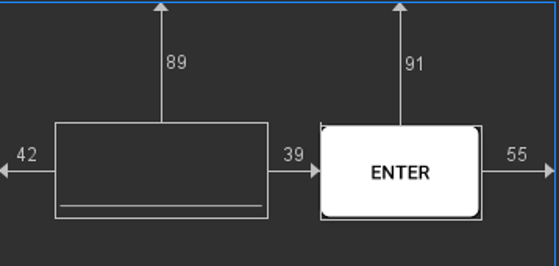
\includegraphics[width=\columnwidth]{img/xml_InputDouble}
	\caption[XML-Designer für die Klassen InputDouble]{XML-Designer für die Klasse InputDouble\footnotemark}
\end{figure}

Die korrespondierende Java-Datei liest nach dem Bestätigen des Buttons den Wert aus dem \code{EditText} und kreiert ein \code{ODouble}-Objekt. Dieses Objekt wird mit seinem zugehörigen \code{TileMapping} einem \code{TileScheme} zugewiesen. Das vorher ausgewählte \code{Tile} aktualisiert seinen \code{TileScheme}. Abschließend schließt der Konstruktor die Dialog über die Methode \code{dismissAll()}, die vorher erklärt wurde.

\paragraph{Klasse: InputFraction [Gentges]}

Diese Klasse deckt die Funktionalität der Benutzereingabe von Brüchen. Dabei ähnelt sie der Klasse InputDouble. Die Unterschiede beruhen dahingehend, dass ein zweites EditText integriert wurde, um sowohl als Zähler als auch Nenner abzufragen. Der ausgewählten Tile wird respektiv ein TileScheme mit OFraction übergeben. 

\begin{figure}[h]
	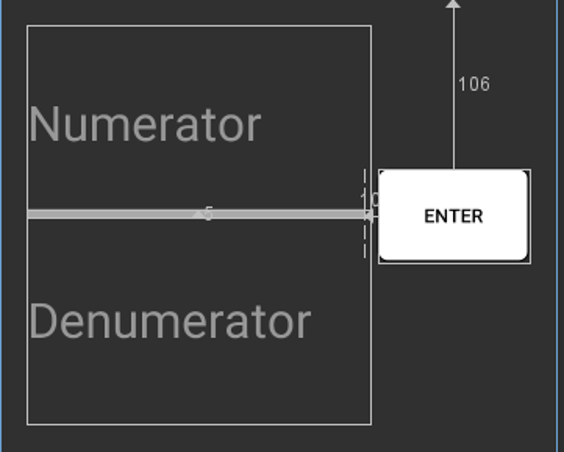
\includegraphics[width=\columnwidth]{img/xml_InputFraction}
	\caption[XML-Designer für die Klasse InputFraction]{XML-Designer für die Klasse InputFraction\footnotemark}
\end{figure}

\paragraph{Klasse: InputPolynomial [Gentges]}

Die Klasse ist grundsätzlich gleich aufgebaut, wie die vorherigen Eingabeklassen der Operanden. In der Abbildung lässt sich erkennen, dass die einzelne Polynome vom Nutzer eingegeben werden können.

\begin{figure}[h]
	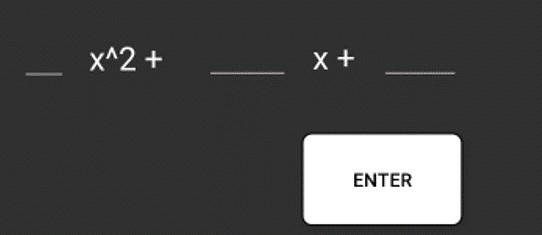
\includegraphics[width=\columnwidth]{img/xml_InputPolynomial}
	\caption[XML-Designer für die Klasse InputPolynomial]{XML-Designer für die Klasse InputPolynomial\footnotemark}
\end{figure}

\paragraph{Klasse: 6.2.5.8	Darstellung der Beziehungen von den Menüsteuerungsklassen [Istogu]}

XXX

\clearpage

\subsection{Dokumentation der Models }

\subsubsection{Operanden [Schwenke]}

Für ein gut funktionierendes Backend ist ein einheitliches Datenmodel essenziell. So gibt es in der Kernbibliothek von Java einige Klassen für die Repräsentation von mathematischen Bausteinen, wie z.B. dem Bruch. Das gleiche gilt für \textit{Apache Commons Math}. 

Jedoch sind die meisten dieser Klassen sehr spezialisiert und miteinander nicht kompatibel. Deswegen wurde innerhalb des Projektteams entschieden für jeden unterstützten Operanden eine eigene Klasse zu entwickeln, die jedoch alle von der gleichen abstrakten Klasse \code{Operand} erben sollen. 

Dadurch wird sichergestellt, dass es eine einheitliche Schnittstelle gibt, über die alle Operanden angesprochen werden können. Beschreiben kann man diese neuen Klassen auch als \textit{Wrapper}, da der Großteil der eigentlichen Funktionalitäten Teil der darunterliegenden Klassen ist. 

So soll z.B. \code{OMatrix} ein Wrapper um die Klasse \code{Array2DRowRealMatrix} sein. Damit kann man einerseits das einfache und einheitliche Interface nutzen und falls notwendig direkt auf das darunterliegende Objekt zugreifen, um spezielle Operationen durchführen zu können. 

Ein wichtiger Bestandteil dieser Wrapper sind auch die unterschiedlichen Konstruktoren. So kann jeder Operand aus einem einzelnen String konstruiert werden. 

Im Folgenden wird die gemeinsame Schnittstelle dargestellt. Gemeinsam haben alle diese Methoden, dass sie ohne Seiteneffekte auskommen. Statt das vorliegende Objekt zu verändern wird ein neues Objekt erstellt und zurückgegeben. Dies macht das Umkehren von Methodenaufrufen einfach. Man muss lediglich das zurückgegebene Objekt entfernen und das alte weiternutzen.

\paragraph{Klasse: Operand [Schwenke]}

\code{Operand turnAroundSign()}: Dreht alle Vorzeichen im Operand um. Erreicht wird das grundsätzlich durch Multiplikation mit \code{-1}. Konkreter muss dafür z.B. bei einer Matrix eine Multiplikation mit einem Skalar durchgeführt werden.

\code{Operand negateValue()}: Negiert den Operanden unabhängig von den Vorzeichen. Bei einer Matrix werden also alle Elemente negativ.

\code{Operand inverseValue()}: Die Inverse (wenn vorhanden) des jeweiligen Operanden wird berechnet.

\code{Boolean equalsValue(Operand o)}: Vergleicht den aktuellen Operanden mit einem übergebenen Operanden.

\code{String toString()}: Wandelt das Objekt in eine String-Repräsentation um.

\code{<T extends Object> get()}: Gibt das darunterliegende Objekt zurück. Im Falle von \code{OMatrix} ist dies eine \code{Array2DRowRealMatrix}. Bei einem Tupel ein \code{Array} von \code{Doubles}.

Auffallend ist hier der geringe Umfang der Schnittstelle der Operanden, da diese doch eigentlich die Grundlage für einen Taschenrechner bilden sollten. So kann man eine Matrix multiplizieren, addieren, dividieren und das alles in unterschiedlichsten Kombinationen mit anderen Arten von Operanden. Tatsächlich sind die meisten Kalkulationen – wie in der Projektplanung entworfen – in eigenen Klassen angelegt. Somit besteht eine Trennung zwischen Datenhaltung (den Operanden) und den Operationen, die auf den Daten ausgeführt werden können (Actions).

\paragraph{Klasse: ODouble [Meinerzhagen]}

\textit{Wrapper für ein \code{Double}}

Eine Dezimalzahl, welche intern einen \code{double} zur Datenspeicherung verwendet.


\paragraph{Klasse: OFraction [Meinerzhagen]}

\textit{Wrapper für Common Math Fraction}

Implementierung eines Bruchs. Die Zähler und Nenner sind durch \code{Doubles} umgesetzt. Im Gegensatz zu den meisten anderen Operanden gibt es hier mehr als zwei Konstruktoren. So kann man einmal Zähler und Nenner als zwei ganze Zahlen übergeben. Wird ein einzelnes \code{Double} übergeben, wird daraus automatisch ein Bruch erstellt. Alternativ kann direkt eine \code{Fraction} übergeben werden.

\paragraph{Klasse: OSet [Meinerzhagen]}

\textit{Wrapper für ein \code{Double}-\code{Set}}

Implementierung einer Menge. Das gleiche Element kann nicht mehrmals enthalten sein. Die Reihenfolge spielt keine Rolle. Umgesetzt ist die Klasse mit einem angepassten \code{Set}. Erstellen kann man ein \code{OSet} aus einem \code{Array} von \code{Doubles} oder einem String.

\paragraph{Klasse: OTuple [Meinerzhagen]}

\textit{Wrapper für ein \code{Double}-\code{Array}}

Implementierung eines Tupels. Das gleiche Element kann mehrmals enthalten sein. Die Reihenfolge spielt eine Rolle. Erstellen kann man ein \code{OTuple} aus einer übergebenen Liste oder einem String.

\paragraph{Klasse: OMatrix [Meinerzhagen]}

\textit{Wrapper für eine Apache Commons \code{Array2DRowRealMatrix}}

Implementierung einer Matrix. Das darunterliegende Objekt ist eine \code{RealMatrix}, die wiederrum eine \code{Array2DRowRealMatrix} enthält. Die Matrix an sich ist in einem zweidimensionalen Array von \code{Doubles} umgesetzt. Erstellen kann man eine \code{OMatrix} aus einem String oder einem zweidimensionalen \code{Array} von \code{Doubles}.


\paragraph{Klasse: OPolynom [Meinerzhagen]}

\textit{Wrapper für eine Apache Commons \code{PolynomialFunction}}

Implementierung eines Polynoms. Grundsätzlich entspricht das Polynom einer einer Sequenz von Dezimalzahlen. Abhängig von der Position in der Sequenz entscheidet sich, was der Exponent der jeweiligen Dezimalzahl ist. Somit müssen Funktionen immer in dieser Normalform vorliegen. Erstellen kann man ein \code{OPolynom} aus einem String oder einem \code{Array} von \code{Doubles}.

\paragraph{Klasse: OEmpty [Meinerzhagen]}

\textit{Leerer Wrapper}

Ein leerer Operand. Da alle \code{Operand}-Klassen Wrapper sind, ist technisch auch ein leerer Wrapper notwendig. Die hier implementierten Methoden aus der Schnittstelle stellen lediglich \textit{Stubs} dar und haben keine Funktion.

\paragraph{Klasse: DoubleFormatter [Meinerzhagen]}

Zentrale Anlaufstelle um \code{Doubles} in einen formattierten String umzuwandeln. Die einzige hier enthaltene Methode ist 

\code{String format(double d)}

\paragraph{Klasse: DoubleComparator [Meinerzhagen]}

Dezimalzahlen sind in den meisten Sprachen in dem IEE 754 Format implementiert. Das hat zur Folge, dass Konversionen und Änderungen einer konkreten Dezimalzahl zu Rundungsfehlern führen. Das ist auch in Java der Fall. Möchte man nun die beiden Dezimalzahlen \code{1.1} und \code{1.1} mit der Standardmethode in Java vergleichen, wird man in fast allen Fällen ein \code{false} zurückbekommen. Das liegt an den zuvor angesprochenen Rundungsfehlern. 

Da innerhalb dieses Projekts alles auf \code{Doubles} basiert ist es notwendig für dieses Problem eine Lösung zu finden. Dafür wurde diese Klasse entwickelt. Alle Vergleiche müssen über diese Klasse erfolgen.

\code{Boolean isEqual(double d1, double d2)} vergleicht zwei \code{Doubles} miteinander. Dies erfolgt über ein Delta. Zunächst wird die Differenz zwischen beiden Zahlen berechnet und anschließend überprüft, ob die Differenz unter einer definierten Grenze liegt. Alle weiteren Methoden in dieser Klasse benutzen diese Methode.

Weitere Methoden vergleichen \code{Arrays} und \code{Sets} miteinander.

\subsubsection{Operationen}

\paragraph{Klasse: Plus [Falk]}

\textbf{Eingabeparameter: }Zwei Werte, der erste Wert ist der erste Summand, der zweite der zweite Summand. Die erlaubten Kombinationen sind: 

\begin{itemize}
	\item \code{ODouble} und \code{ODouble}
	\item \code{ODouble} und \code{OFraction}
	\item \code{OFraction} und \code{ODouble}
	\item \code{ODouble} und \code{OSet}
	\item \code{OSet} und \code{ODouble}
	\item \code{ODouble} und \code{OMatrix}
	\item \code{OMatrix} und \code{ODouble}
	\item \code{ODouble} und \code{OPolynom}
	\item \code{OPolynom} und \code{ODouble}
	\item \code{ODouble} und \code{OTupel}
	\item \code{OTupel} und \code{ODouble}
	\item \code{OFraction} und \code{OFraction}
	\item \code{OFraction} und \code{OSet}
	\item \code{OSet} und \code{OFraction}
	\item \code{OFraction} und \code{OMatrix}
	\item \code{OMatrix} und \code{OFraction}
	\item \code{OFraction} und \code{OPolynom}
	\item \code{OPolynom} und \code{OFraction}
	\item \code{OFraction} und \code{OTuple}
	\item \code{OTupel} und \code{OFraction}
	\item \code{OMatrix} und \code{OMatrix}
	\item \code{OPolynom} und \code{OPoylnom}
	\item \code{OTuple} und \code{OTuple}
\end{itemize}

\textbf{Rückgabewerte: }Der berechnete Wert mit dem Datentyp des ersten Summanden. 

\textbf{Beschreibung: }Die Klasse verfügt über 23 öffentlich ansprechbare Methoden. Je nach übergebenen Parametern wird bestimmt, welche öffentliche Methode gemeint ist. Anschließend wird die Berechnung durchgeführt. 

\paragraph{Klasse: Minus [Falk]}

\textbf{Eingabeparameter: }Zwei Werte, der erste Wert ist der Minuend, der zweite der Subtrahend. Die erlaubten Kombinationen sind: 

\begin{itemize}
	\item ODouble und ODouble 
	\item ODouble und OFraction
	\item OFraction und OFraction 
	\item OFraction und ODouble 
	\item OSet und ODouble
	\item OSet und OFraction 
	\item OMatrix und OMatrix
	\item OMatrix und ODouble
	\item OMatrix und OFraction
	\item OPolynom und OPolynom 
	\item OPolynom und ODouble
	\item OPolynom und OFraction 
	\item OTuple und OTuple
	\item OTuple und ODouble
	\item OTuple und OFraction
\end{itemize} 

\textbf{Rückgabewerte: }Der berechnete Wert mit dem Datentyp des ersten, übergebenen Wertes. 

\textbf{Beschreibung: }Die Klasse verfügt über 15 öffentlich ansprechbare Methoden. Je nach übergebenen Parametern wird bestimmt, welche öffentliche Methode gemeint ist. Anschließend wird die Berechnung durchgeführt. 

\paragraph{Klasse: Minus [Falk]}

\textbf{Eingabeparameter: }Zwei Werte, der erste Wert ist der Dividend, der zweite der Divisor. Die erlaubten Kombinationen sind: 

\begin{itemize}
	\item ODouble und ODouble
	\item ODouble und OFraction
	\item OFraction und OFraction 
	\item OFraction und ODouble 
	\item OSet und ODouble
	\item OSet und OFraction
	\item OMatrix und ODouble 
	\item OMatrix und OFraction
	\item OPolynom und OPolynom 
	\item OPolynom und ODouble
	\item OPolynom und OFraction 
	\item OTuple und OTuple
	\item OTuple und ODouble
	\item OTuple und OFraction 
\end{itemize}

\textbf{Rückgabewerte:} Der berechnete Wert mit dem Datentyp des ersten, übergebenen Wertes.
 
\textbf{Beschreibung: }Die Klasse verfügt über 14 öffentlich ansprechbare Methoden. Je nach übergebenen Parametern wird bestimmt, welche öffentliche Methode gemeint ist. Bevor die Berechnung durchgeführt wird, wird bestimmt ob der Divisor null ist. Wenn ja wird eine Fehlermeldung ausgegeben. Andernfalls wird die Berechnung durchgeführt. 

\paragraph{Klasse: Times [Falk]}

\textbf{Eingabeparameter: }Zwei Werte, der erste Wert ist der Multiplikator, der zweite Wert der Multiplikand. Die erlaubten Kombinationen sind: 

\begin{itemize}
\item ODouble und ODouble
\item ODouble und OFraction
\item OFraction und ODouble
\item ODouble und OSet
\item OSet und ODouble
\item ODouble und OMatrix
\item OMatrix und ODouble
\item ODouble und OPolynom
\item OPolynom und ODouble
\item ODouble und OTupel,
\item OTupel und ODouble
\item OFraction und OFraction
\item OFraction und OSet
\item OFraction und OMatrix
\item OMatrix und OFraction
\item OFraction und OPolynom
\item OFraction und OTupel
\item OMatrix und OMatrix
\item OPolynom und OPolynom 
\item OTupel und OTupel 
\end{itemize}

\textbf{Rückgabewerte: }Der berechnete Wert. 

\textbf{Beschreibung: }Die Klasse verfügt über 20 öffentlich ansprechbare Methoden. Je nach übergebenen Parametern wird bestimmt, welche öffentliche Methode gemeint ist. Anschließend wird die Berechnung durchgeführt. 

\paragraph{Klasse: Root [Falk]}

\textbf{Eingabeparameter: }Zwei Werte, der erste Wert ist der Radikand, der zweite Wert der Wurzelexponent. Die erlaubten Kombinationen sind: 

\begin{itemize}
\item ODouble und ODouble
\item ODouble und OFraction
\item OFraction und ODouble 
\item OFraction und OFraction
\item OMatrix und ODouble
\item OMatrix und OFraction
\end{itemize}

\textbf{Rückgabewerte:} Der berechnete Wert, Datentyp ist der des Radikanden. 

\textbf{Beschreibung: }Die Klasse verfügt über 6 öffentliche Methoden. Anhand der übergebenen Parameter wird bestimmt, welche öffentliche Methode aufgerufen wird. In der Methode wird die Wurzel berechnet und zurückgegeben. 

\paragraph{Klasse: Modulo [Falk]}

\textbf{Eingabeparameter:} Zwei Werte des Typs \code{ODouble}, der erste Wert ist der Dividend, der zweite der Divisor. 

\textbf{Rückgabewerte:} Der berechnete Wert als \code{ODouble}. 

\textbf{Beschreibung:} Die Klasse verfügt über eine öffentliche Methode. In der Methode wird der Modulo-Wert der beiden übergebenen Parameter berechnet. 

\paragraph{Klasse: Zeros [Keienburg]}

\textbf{Eingabeparameter: }Eine Funktion des Typs \code{OPolynom}

\textbf{Rückgabewerte:} Ein Set des Typs \code{OSet} mit den berechneten Nullstellen. Die Nullstellen werden als \code{Set} zurückgegeben, da so verhindert wird das für Funktionen wie \code{x\^2+0*x+0} zweimal die gleiche Nullstelle zurückgegeben wird. 

\textbf{Einstieg in die Klasse:} Öffentliche Methode, die die übergebenen Parameter entgegennimmt. Die weiteren Methoden für die Berechnung werden anschließend von der Öffentlichen Methode aus aufgerufen. 
Methoden der Klasse \code{Zeros}:

\code{calculateZeros}: Die Methode erhält eine Funktion vom Typ \code{OPolynom}. Anschließend wird bestimmt, von welchem Grad die übergebene Funktion ist. Wenn die Funktion ersten Grades ist, wird die Methode \code{zerosTypeOne} aufgerufen, ansonsten die Methode \code{zerosTypeTwo}. Die beiden Methoden geben die gefundenen Nullstellen als 
Array zurück, das Array wird anschließend von \code{calculateZeros} zurückgegeben.
 
\code{normalOrQuadraticFunction}: Bestimmt, ob eine, als \code{Double} Array übergebene Funktion, ersten oder zweiten Grades ist. Dabei wird die Länge des Arrays getestet. Ist die Länge des Arrays 3, so wird die Funktion als Quadratische Funktion bestimmt. Wenn die Länge 2 ist, als einfache Funktion. 

\code{zerosTypeOne}: Die Methode berechnet die Nullstellen für Funktionen ersten Grades. Die Funktion wird als Double Array übergeben. Die berechnete Nullstelle wird als Double Array zurückgegeben. 

\code{zerosTypeTwo}: Die Methode berechnet die Nullstellen für Funktionen zweiten Grades. Die Funktion wird als Double Array übergeben. Mithilfe der Mitternachtsformel wird die erste und die zweite Nullstelle bestimmt. Die gefundenen Nullstellen werden als Double Array zurückgegeben. 

\textbf{Anmerkung:} Wenn eine übergebene Funktion keine Nullstellen besitzt, der Rückgabewert in Java also \code{NaN} ist, wird eine Fehlermeldung ausgegeben, dass eine Nullstellenberechnung nicht möglich ist. 

\textbf{Einschränkungen:} Die Nullstellenberechnung ist nur für Funktionen ersten und zweiten Grades möglich. 

Unit-Tests für die Klasse: 

\begin{enumerate}
	\item Eingabe Funktion: \code{2x + 4}. Erwartetes Ergebnis: \code{(-2)}
	\item Eingabe Funktion: \code{2x\^{}2+4x+0}. Erwartetes Ergebnis: \code{(-2, 0)}
	\item Eingabe Funktion: \code{x\^{}2+4x-4}. Erwartetes Ergebnis: \code{(-4,828, 0,828)}
\end{enumerate}

Die Tests waren erfolgreich.

\paragraph{Klasse: HighAndLowPoints [Keienburg]}

\textbf{Eingabeparameter:} Eine Funktion des Typs \code{OPolynom}

\textbf{Rückgabewerte: }Ein Tupel des Typs \code{OTupel} mit den berechneten Extremwerten. Die Werte an den geraden Positionen innerhalb des Tupels sind die X-Werte, der jeweils folgende Wert ist der zugehörige Y-Wert. Bsp.: Tupel [0] = X-Wert des ersten Extremwertes, Tupel [1] = Y-Wert des ersten Extremwertes, Tupel [2] = X-Wert des zweiten Extremwertes, Tupel [3] = Y-Wert des zweiten Extremwertes. 

Beschreibung: Die Klasse erhält eine Funktion vom Typ \code{ODouble}. Zuerst wird die Ableitung der Funktion bestimmt, anschließend die Nullstellen der Abteilung. Für die erhaltenen Nullstellen wird der zugehörige Y-Wert berechnet. Die berechneten Werte werden als \code{OTupel} zurückgegeben. 

Einstieg in die Klasse: Öffentliche Methode, die die übergebenen Parameter entgegennimmt. Die weiteren Methoden für die Berechnung werden anschließend von der Öffentlichen Methode aus aufgerufen. 

\textbf{Methoden der Klasse \code{HighAndLowPoints}:}

\code{getHighAndLowPoints}: Einstiegspunkt der Klasse, ruft die Methode \code{calculateHighAndLowPoints} für die weitere Berechnung der Extremwerte auf. Gibt sie als Double Array zurück. 

\code{getFunctionAsDouble}: Wandelt eine übergebene Funktion vom Typ \code{OPolynom} in ein Double Array um.

\code{calculateHighAndLowPoints}: Berechnet die Nullstellen einer übergebenen Funktion vom Typ \code{OPolynom}. Berechnet zuerst die Ableitung der Funktion, anschließend die Nullstellen der Ableitung. Die Werte der Nullstellen werden anschließend in die ursprüngliche Funktion eingesetzt und so die Y-Werte berechnet. Die berechneten Nullstellen werden als Double Array zurückgegeben. 

\code{Einschränkungen}: Die Nullstellenberechnung ist nur für Funktionen zweiten Grades möglich. Demnach ist eine Berechnung der Hoch- und Tiefpunkte nur für Funktionen dritten oder zweiten Grades möglich.

Unit-Tests für die Klasse:

\begin{itemize}
\item Eingabe Funktion: 2x\^{}2+4x+6. Erwartetes Ergebnis: (-1|4)
\item Eingabe Funktion: 3x\^{}2+6x-4. Erwartetes Ergebnis: (-1|-7)
\item Eingabe Funktion: -2*x\^{}2+4x+12. Erwartetes Ergebnis: (1|14)
\end{itemize}

Die Tests waren erfolgreich.

\paragraph{Logarithm [Keienburg]}

\textbf{Eingabeparameter:} Ein Wert des Typs ODouble oder zwei Werte vom Typ ODouble (erster ist die Basis) 

\textbf{Rückgabewerte:} Ein Wert des Typs ODouble

\textbf{Beschreibung:} Die Klasse berechnet den Logarithmus. Die Art des Logarithmus ist abhängig von den übergebenen Parametern. Wird nur ein Wert übergeben, wird der natürliche Logarithmus der Zahl berechnet. Wenn zwei Parameter übergeben werden, ist der erste Parameter die Basis des Logarithmus, der zweite der Wert, zu für den der Logarithmus berechnet werden soll. 

Der Einstieg in die Klasse erfolgt über zwei öffentliche Methoden. Die Methode wird anhand der übergebenen Parameter (ein oder zwei Werte vom Typ \code{ODouble}) ausgewählt. In der Öffentlichen Methode findet die Berechnung des Logarithmus (Natürlicher oder Logarithmus zu einer bestimmten Basis) statt. Wenn ein Wert kleiner gleich null eingegeben wird, wird eine Fehlermeldung ausgegeben.

Unit-Tests für die Klasse: 4 Unit-Test für die Berechnung der des natürlichen Logarithmus (ersten 4), 3 Unit-Tests für die Berechnung des Logarithmus für eine beliebige Basis. 

\begin{itemize}
\item Eingabe 10. Erwartetes Ergebnis: 2.302585092994046
\item Eingabe: 5. Erwartetes Ergebnis: 1.6094379124341003
\item Eingabe: 97. Erwartetes Ergebnis: 4.574710978503383
\item Eingabe: e. Erwartetes Ergebnis: 1
\item Eingabe: Basis 5, Wert 10. Erwartetes Ergebnis: 1.4306765580733933
\item Eingabe: Basis 10, Wert 10. Erwartetes Ergebnis: 1
\item Eingabe: Basis e, Wert 10. Erwartetes Ergebnis: 2.302585092994046
\end{itemize}

Die Tests waren erfolgreich.

\paragraph{Logarithm10 [Keienburg]}

\textbf{Eingabeparameter:} Ein Wert des Typs ODouble

\textbf{Ausgabeparameter:} Ein Wert des Typs ODouble

\textbf{Beschreibung:} Die Klasse berechnet den Logarithmus zur Basis 10. Wenn ein Wert kleiner gleich null eingegeben wird, wird eine Fehlermeldung ausgegeben. 

Unit-Tests für die Klasse: 

\begin{itemize}
\item Eingabe 10. Erwartetes Ergebnis: 1
\item Eingabe: 5. Erwartetes Ergebnis: 0.6989700043360189
\item Eingabe: 97. Erwartetes Ergebnis: 1.9867717342662448
\end{itemize}

Die Tests waren erfolgreich.

\paragraph{Derivation [Keienburg]}

\textbf{Eingabeparameter: }Eine Funktion des Typs OPolynom

\textbf{Rückgabewert:} Eine Funktion des Typs OPolynom

\textbf{Beschreibung:} Die Klasse berechnet die Ableitung zu einer übergebenen Funktion des Typs OPolynom und gibt sie als Funktion vom Typ OPolynom zurück. 

\textbf{Einstieg in die Klasse: }Öffentliche Methode, die die übergebenen Parameter entgegennimmt. Die weiteren Methoden für die Berechnung werden anschließend von der Öffentlichen Methode aus aufgerufen. 

\textbf{Methoden der Klasse Derivation: }

\code{getFunctionAsDouble:} Wandelt eine gegebene Funktion vom Typ OPolynom in ein Double Array um. 

\code{derivate: }Berechnet die Ableitung einer gegebenen Funktion. Die Funktion wird zuerst in ein Double Array umgewandelt, anschließend abgeleitet und als Funktion vom Typ OPolynom zurückgegeben. 

Unit-Tests für die Klasse: 

\begin{itemize}
\item Eingabe 2x\^{}2+4x+6. Erwartetes Ergebnis: 4x+4
\item Eingabe: 7x+9. Erwartetes Ergebnis: 7
\item Eingabe: 12x\^{}2-3+12. Erwartetes Ergebnis: 24x-1
\item Eingabe: 1.5x\^{}2+2x+7. Erwartetes Ergebnis: 2.25x+2
\end{itemize}  

Die Tests waren erfolgreich.

\paragraph{Integral [Istogu]}

Diese Klasse erbt von der Klasse ‘‘Action’‘. Daher sind die Methoden „with()“ bereits implementiert. Diese Klasse berechnet entweder die Stammfunktion von dem übergebene Polynomialfunktion oder das Integral der Funktion. 

Für die Bildung der Stammfunktion benötigt die Methode „getAntiderivative()“ eine „OPolynom“ und gibt die Stammfunktion als Typ „OPolynom“ zurück. Beim „Aufleiten“ entsteht eine Konstante, die jede Wert annehmen kann. In der App wird festgelegt, dass diese Konstante immer 0 ist. Zweck hinter der Definition ist, dass mit dem OPolynom weitergerechnet werden kann, da diese nicht mit weiteren Variablen arbeiten kann.

Für das Berechnen des Integrals getSimpsonIntegrator() werden folgende Parametertypen erwartet: OPolynom oPolynom, double lowerBound, double upperBound. Das Integral für den vorgegebenen Bereich wird als ODouble zurückgegeben. Diese Methode realisiert die Simpsonregel für die Integration von realen Funktionen, die in dem genutzten Mathebibliothek als Klasse SimpsonIntegrator implementiert wurde. 

Nach der Implementierung der Klasse erstellte ich dazu gehörig eine Unit-Test-Klasse. Im Nachfolgenden werden die Ergebnisse dargestellt, die alle erfolgreich waren. 

\code{getSimpsonsIntegrator()}
\quad 1.	Eingabe: OPolynom: x\^{}2 – 8x + 17, untere Grenze: 2, obere Grenze 5

\quad Erwartetes Ergebnis: 6

\code{getAntiderivative()}
1.	Eingabe: OPolynom: -3,21x\^{}3 + 3x + 7
Erwartetes Ergebnis: OPolynom: -0,8025x\^{}4 + 1,5x\^{}2 + 7x + c

\textbf{Bestimmung des Grenzwertes einer Funktion [Istogu]}

Für die Umsetzung wurde die Funktion ‘‘value(double x)’‘ der Klasse ‘‘PolynomialFunction’‘ verwendet, die aus der Mathebibliothek ‘‘Apache Commons Math’‘ hervorgeht. Zudem bietet die Double-Klasse die Repräsentierung von positiv und negativ Unendlich an, die auch für die Methoden verwendet wurde.

Für die Bestimmung des Grenzwertes wurde sich an der Methode der numerischen Annäherung orientiert. Hierbei wird der Grenzwert durch die Annäherung von links und rechts des untersuchten Punktes bestimmt. Daher wurde die Anforderung in drei Methoden untergliedert, einmal die Methode ‘‘limitFromBelow(…)’‘ und ‘‘limitFromAbove(…)’‘, die jeweils die Annäherung von verschiedenen Richtung bestimmt. Die Rückgabewerte der beiden Methoden werden in der Methode ‘‘limit(…)’‘ miteinander verglichen. Zweck der Vergleichsabfrage ist es Definitionslücken abzufangen. Als Beispiel wird folgende Funktion angenommen:

f(x)=1/x

\begin{figure}[!h]
	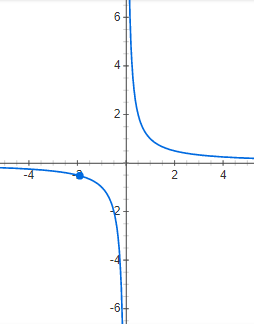
\includegraphics[scale=1]{img/funktion-grafik}
	\caption[Grafische Darstellung der Funktion]{Grafische Darstellung der Funktion\footnotemark}
\end{figure}
\footnotetext{eigene Darstellung}

Wenn für die Funktion sowohl der linksseitige als auch der rechtsseitige Grenzwert bestimmt wird, folgt folgendes:  
































\subsection{Überblick über die Activities der App bzw. der Funktionen}

\subsection{Dokumentation der Navigation zwischen Activities}

\subsection{Dokumentation der Activity-übergreifenden, persistenten Datenhaltung}

\subsection{Dokumentation der programmatischen Beiträge der Teammitglieder}

\subsubsection{Tom Bockhorn}

\newpage

\subsubsection{Hendrik Falk}

\newpage

\subsubsection{Dennis Gentges}

\newpage

\subsubsection{Getuart Istogu}

\newpage

\subsubsection{Jannis Keienburg}

\newpage

\subsubsection{Tim Jonas Meinerzhagen}

\newpage

\subsubsection{Khang Pham}

\newpage

\subsubsection{Tim Schwenke}

\para{Generische Kalkulationsorchestrierung}

Wie schon im Kapitel zur Projektplanung erwähnt, stellt die Strukturierung und Architektur der Rechnungsumsetzung im Backend eine der vielen Anforderungen des Projekts dar. Identifiziert wurden zwei Hauptarten von Kalkulationen. 

Die erste Art ist generisch und wird in einer großen Anzahl benötigt. Ein Beispiel dafür ist die Addition. Da der Taschenrechner viele unterschiedliche Operanden-Typen unterstützt (Matrizen, Brüche, Mengen, usw.) sind enorm viele Methoden notwendig, um alle Möglichkeiten der Addition abdecken zu können. Auch muss irgendwo vom Programm entschieden werden, welche Methode genau aufgerufen werden soll. Statt dies mit komplexen If-Else-Bedingungen zu lösen, wurde in der Planungsphase entschieden Reflektion zu nutzen. Somit kann man in sich geschlossene kleine Methoden programmieren, die - sofern die Schnittstellenanforderungen erfüllt sind - automatisch erkannt und von der Reflektionsmethode aufgerufen werden können. Der Nutzer im Frontend muss lediglich entscheiden, was für eine Art von generischer Kalkulation er ausführen möchte. Zum Beispiel Addition oder Multiplikation. 

Die zweite Art von Kalkulationen sind sehr spezifisch, z.B. ein bestimmter Algorithmus zum Lösen von kubischen Gleichungen. Hier sind keine/kaum Kombinationen möglich und können somit direkt aufgerufen werden, ohne Reflektion zu verwenden.

Implementiert ist die Reflektion in der abstrakten Klasse \code{Action}. Die Klassenvariable \code{scopedAction} zeigt zur Laufzeit auf eine konkrete Implementierung einer \code{Action}, also z.B. \code{Plus}. Auf \code{scopedAction} wird die Reflektion ausgeführt. Letztere ist in der Methode \code{with()} umgesetzt. Diese stellt die Schnittstelle zu den generischen Kalkulationen erster Art dar. Hier ist der Methodenkopf zu sehen:

\begin{figure}[bht]
	\begin{lstlisting}[
	caption=Methodenkopf der generischen Schnittstelle,
	label=list:methodenkopf-der-generischen-schnittstelle,
	language=Java]
@Contract(pure = true) public @NotNull 
Operand with(@NotNull Operand... operands) 
throws CalculationException
	\end{lstlisting}    
\end{figure}

Die erste Zeile definiert einige Eigenschaften der Methode. \code{@Contract} sagt aus, dass die Funktion \textit{pure} ist. Sie gibt für Tupel von Operanden immer das gleiche Ergebnis zurück und ist grundsätzlich ohne Nebeneffekte. Das ist hilfreich für das automatische Testen. Als Parameter wird ein beliebig gro"ses Array von Operanden übergeben. Das Ergebnis ist immer eine valide Instanz von \code{Operand}. Wird versucht eine nicht unterstützte Kalkulation auszuführen, wird \code{CalculationException} geworfen. Diese Ausnahme ist keine \code{RunTimeException} und muss deswegen explizit behandelt werden. Alternativ hätte man hier auch Optionals nutzen. Jedoch unterstützt die genutzte Version der Android API dieses Java-Feature nicht.

\begin{figure}[bht]
	\begin{lstlisting}[
	caption=Implementierung der generischen Schnittstelle,
	label=list:implementierung-der-generischen-schnittstelle,
	language=Java]
Class[] operandClasses = new Class[operands.length];
Operand resultOperand;

for (int i = 0; i < operands.length; i++)
	operandClasses[i] = operands[i].getClass();

try {
	resultOperand = (Operand) scopedAction.getClass()
		.getDeclaredMethod("on", operandClasses)
		.invoke(scopedAction, (Object[]) operands);
} catch (SeveralExceptions e) {
	throw new CalculationException(e.getMessage());
}

if (resultOperand != null) return resultOperand;
else throw new CalculationException();
	\end{lstlisting}    
\end{figure}

Die Reflektion in Listing~\ref{list:implementierung-der-generischen-schnittstelle} beginnt mit der Extraktion der Klasse jedes übergebenen Operands. Das kann z.B. die Klasse \code{Matrix} oder \code{Fraction} sein, die alle von \code{Operand} erben. Die extrahierten Klassen werden in Array \code{operandClasses} gespeichert. Die hier vorliegende Sequenz liefert die Antwort auf die Frage, welche konkrete Methode aufgerufen werden soll. Die Entscheidung basiert alleine auf dieser Sequenz und der konkreten \code{Action} auf die \code{scopedAction} zeigt. Aus letzterer Variable wird die Klasse extrahiert und die Methode \code{getDeclaredMethod()} aufgerufen. Damit kann man eine Methode in einer Klasse auf Basis des Namens (in unserem Falle immer \code{on}) und eine Sequenz von Parametertypen finden. Diese wird anschlie"send mit \code{invoke()} aufgerufen, wobei die Operanden übergeben werden. Kommt es zu einem Fehler werden alle Fehlertypen in \code{CalculationException} zusammengefasst und weitergegeben. Ansonsten wird das Ergebnis zurückgegeben.

\newpage












\subsection{Beschreibung von Problemen}

\para{Nutzung von Stack für Notation [Schwenke]}

Der Taschenrechner soll als Eingabelogik für die Anwendung von Operationen die umgekehrte polnische Notation verwenden. Hierbei werden immer zunächst die Operanden und im Anschluss daran die darauf auszuführenden Operatoren angegeben. Dieser Ansatz ermöglicht eine stapelbasierte Abarbeitung. 

Stacks werden, wie von den meisten Programmiersprachen, auch in Java in der Standardbibliothek unterstützt. Mit dabei sind Methoden wie \code{push} (für das Ablegen eines Objekts auf dem Stapel), \code{pop} (für das Entfernen und die Wiedergabe eines Objekts auf dem Stapel), \code{peek} (für die Wiedergabe ohne Entfernen eines Objekts auf dem Stapel) und \code{empty} (für das Leeren des Stapels). 

Jedoch müssen hierbei die besonderen Anforderungen des Taschenrechners beachtet werden. Operanden können von gänzlich unterschiedlichem Typus sein, zum Beispiel eine einfache Dezimalzahl oder auch ein Tupel, und viele Operationen benötigen mehr als die ersten (maximal zwei) Operanden auf dem Stack. Möchte man Elemente vom Stapel entfernen, kann man \code{pop} mehrmals aufrufen. Aufwändiger hingegen wird es bei \code{peek}. Möchte man mehrere Elemente vom Stapel einsehen ohne diese zu entfernen, muss man bei der Arbeit mit dem vorhandenen Stack einen weiteren bereithalten, nur um zwischengespeicherte Elemente lagern zu können. Anders ist es nicht möglich \code{peek} auf mehrere Elemente gleichzeitig anzuwenden. Gerade das ist aber bei der App notwendig. Weitere Methoden, die bei der umgekehrten polnischen Notation oft benötigt werden, aber nicht implementiert sind, sind \code{reverse} (für die Vertauschung der ersten zwei Elemente auf dem Stack, was wichtig für nicht-kommutative Operationen ist), \code{rollUp} (das unterste Elemente wird an den ersten Platz geschoben, das erste Element an den zweiten Platz usw.) und \code{rollDown} (das unterste Elemente wird an den ersten Platz geschoben, das erste Element an den zweiten Platz usw.).

Aufgrund dessen soll für dieses Projekt ein eigener Stapel implementiert werden. Dieser soll die zuvor genannten Funktionen mit unterschiedlichen Parametertypen unterstützen. Dabei ist darauf zu achten, dass die Programmierung generisch erfolgt und das Stack nicht nur alle Typen von Operanden unterstützt, sondern auch für gänzlich andere Klassenbäume in der App verwendet werden kann.

\para{Ansatz der Kalkulationsorchestrierung [Schwenke]}

Die App soll den Umgang mit unterschiedlichen Operanden-Typen beherrschen. Die Addition zweier Matrizen funktioniert anders als die Addition von zwei einfachen Dezimalzahlen. Java verfügt nativ weder über die entsprechenden Operanden noch über die Methoden für die Kalkulation. Auch die ausgewählte Bibliothek ist nicht ohne weiteres in der Lage Operationen auf alle Kombinationen von Operanden im folgenden Format einheitlich anzuwenden:

\begin{figure}[bht]
	\begin{lstlisting}[caption=Konzept für Nutzung generischer Schnittstelle, label=list:konzept-fuer-nutzung-generischer-schnittstelle]
	Operation.mit(matrixOperand, dezimalOperand, dezimalOperand)
	\end{lstlisting}    
\end{figure}

Einheitlichkeit ist notwendig, damit im Frontend der Applikation keine Logik vorhanden sein muss, die entscheidet wie genau (auf Basis der Operanden-Typen) eine Operation umgesetzt wird. Deswegen muss eine einfache Schnittstelle entwickelt werden, die für den Nutzer nur zwei Drehschrauben bereitstellt. Dies ist zunächst die Auswahl der gewünschten Operation. Das kann z.B. das Symbol \code{+} als übliches Zeichen für Addition sein. Anschließend wird eine Reihe von Operanden übergeben. Dieser Aufruf sollte schließlich das Ergebnis in Form eines Operanden zurückgeben. Im Fall der Addition einer Matrix mit einer rationalen Zahl wäre dies wiederrum eine Matrix. Die korrekte Kalkulation soll also dynamisch bestimmt werden. Wichtig zu klären ist hier auch das Verhalten im Falle eines Fehlschlags. Nicht alle Kombinationen von Operanden können unterstützt werden. Die Verwendung von \textit{Optionals} (ein \code{Optional} ist ein Objekt, das man sich als Datenbehälter vorstellen kann, der entweder einen Wert enthält oder leer – aber nicht \code{null} sein kann) bietet sich hier zwar an, wird jedoch von Java in der verwendeten Android API-Version nicht unterstützt. Deswegen ist hier geplant sogenannte \textit{checked Exceptions} zu verwenden. Diese müssen bei der Verwendung explizit aufgefangen und weiterverarbeitet werden. Die Abbildung einer Operanden-Kombination auf die entsprechende konkrete Kalkulationsmethode muss dementsprechend zur Laufzeit des Programms erfolgen. Ein solches Mapping ist in Java nur mithilfe des Reflection-Pakets möglich. Reflektion ermöglicht den Einblick in ein Objekt (neben der Nutzung des Punkt-Operators) in eine Klasse. Zum Beispiel kann man eine Methode anhand einer Kombination von Parametertypen finden und aufrufen. Es ist geplant diesen Ansatz für die Orchestrierung der Kalkulationen in der App zu verwenden. Auch ist es nicht notwendig nur eine vordefinierte Anzahl an Argumente anzunehmen. So kann es sinnvoll sein, dass eine Methode zur Erstellung eines Tupels eine beliebige Anzahl an Operanden annimmt. Auch das lässt sich mit Reflektion umsetzen.

Der große Vorteil dabei ist, dass nirgendwo explizit in einer Abfrage entschieden werden muss, welche Kombination von Operanden an welche Methode weitergeleitet werden soll. Die Zuordnung erfolgt rein über die Deklaration der Parametertypen in der Methode selbst. Das macht das Ändern und Erweitern der Rechenfunktionalitäten einfach. Es muss lediglich die entsprechende Klasse herausgesucht und eine Methode im korrekten Format hinzugefügt werden. 

Zu entscheiden ist ebenfalls, ob das Gros der Rechenmethoden innerhalb der jeweiligen Operanden-Klassen oder dedizierten Klassen für die Kalkulation angesiedelt sind. Die erste Option hat neben der stärkeren Objektorientierung den Vorteil, dass immer klar ist, dass eine Methode mit den übergebenen Argumenten auf dem jeweiligen Objekt ausgeführt wird. Andererseits erhöht dies die Komplexität der Operanden-Klassen deutlich. Unterstützt man wie geplant 5 bis 7 dedizierte Typen von Operanden und 10 Kalkulationsarten, muss jede Klasse potenziell dutzende Methoden für die Rechnung enthalten. Die andere, und bevorzugte Option, ist die Auslagerung der Kalkulationsmethoden in eigenständige Klassen. Dies reduziert zwar nicht die Anzahl benötigter Methoden, isoliert die Rechenlogik jedoch in Klassen. Innerhalb dieser Klassen wird prozedural programmiert.  Eine typische Charakteristik von Objekten und deren Methoden ist \textit{Mutability}. Eine Methode bekommt ein Objekt und kann dieses verändern. Dies kann Testen unter Umständen aufwändiger gestalten. Durch Isolierung der Rechnungen in eigenen Klassen kann hingegen sichergestellt werden, dass jede Methode \textit{immutable}, also unveränderlich, ist. Das macht das Schreiben von Tests einfach. In Java kann Immutability durch die Verwendung von Annotationen sichergestellt werden. 



